\documentclass{standalone}

\usepackage{tikz}

\usetikzlibrary{positioning, arrows}

\begin{document}

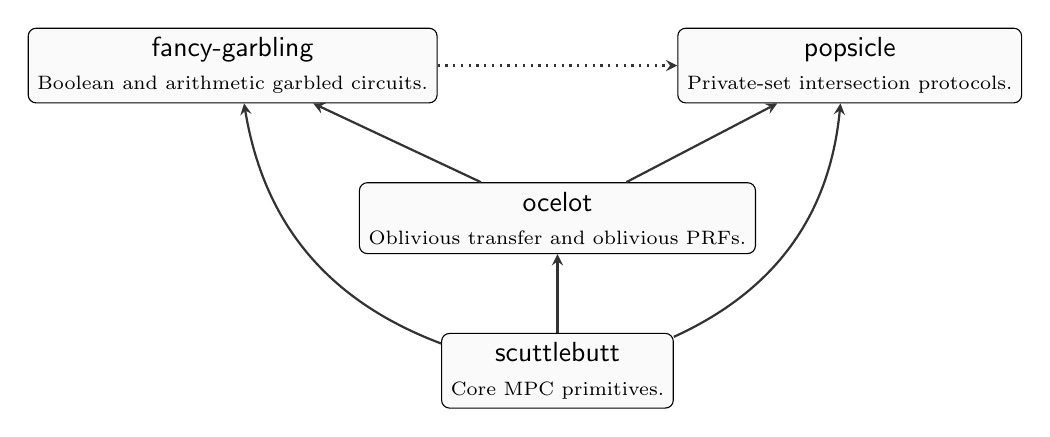
\begin{tikzpicture}
    [every node/.style={draw, align=center, rounded corners=.1cm, fill=black!2},
     arr/.style={draw=black!80, thick, >=stealth, ->},
    ]
    \node (scuttlebutt) {
        \textsf{scuttlebutt}\\
        \scriptsize
        Core MPC primitives.
    };
    \node (ocelot) [above=of scuttlebutt] {
        \textsf{ocelot}\\
        \scriptsize
        Oblivious transfer and oblivious PRFs.
    };
    \node (fancy-garbling) [above left=1cm and -1cm of ocelot] {
        \textsf{fancy-garbling}\\
        \scriptsize
        Boolean and arithmetic garbled circuits.
    };
    \node (popsicle) [above right=1cm and -1cm of ocelot] {
        \textsf{popsicle}\\
        \scriptsize
        Private-set intersection protocols.
    };

    \draw [arr] (scuttlebutt) to [bend left] (fancy-garbling);
    \draw [arr] (scuttlebutt) to [bend right] (popsicle);
    \draw [arr] (scuttlebutt) -- (ocelot);

    \draw [arr] (ocelot) -- (popsicle);
    \draw [arr] (ocelot) -- (fancy-garbling);

    \draw [arr, dotted] (fancy-garbling) -- (popsicle);

\end{tikzpicture}

\end{document}
